\section{Literature Review}

\subsection{Existing solutions}

	\subsubsection{Group Chat-Based Systems (Current Solution at VGU)}
		Currently, many educational institutions, including VGU, rely on informal systems like social media group chats (e.g., Facebook or WhatsApp groups) for raising support tickets and contacting staff. While these systems are easy to set up and require minimal resources, they suffer from significant limitations:
		
		\begin{itemize}
			\item[-] \textbf{Lack of Structure}: The conversation threads are disorganized, making it hard to track specific issues or prioritize them.
			
			\item[-] \textbf{Absence of Accountability}: There’s no formal ticketing system, leading to delays in responses and no mechanism to track whether an issue has been resolved.
			
			\item[-] \textbf{Inadequate Historical Data}: It's difficult to retrieve past conversations or analyze data to improve service.
			
			\item[-] \textbf{Lack of Privacy}: Group chats often expose personal information to all participants, which may raise privacy concerns.
		\end{itemize}
		
		
		\subsubsection{Existing University and Open-source Ticketing Systems}
		Several universities have adopted formal ticket management systems for handling student support services. These systems are often integrated into larger university management platforms or custom-built web applications. Common examples include:
		
		\begin{longtable}{{|l|m{6cm}|m{6cm}|}} 
			\hline
			\textbf{Systems} & \textbf{Features} &\textbf{Limitations}\\ \hline
			\endhead
			JIRA Service Management 
			& Offers customizable workflows, automated prioritization, and detailed issue tracking.
			& Too complex for university needs, expensive, and difficult to adapt without major customization.
			\\ \hline
			Freshdesk 
			& Supports ticket management, multi-channel communication, and agent collaboration. 
			& Feature-heavy and expensive for universities; lacks educational-specific tools.
			\\ \hline
			Zendesk 
			&  Provides email, live chat, and ticketing, with automation and analytics. 
			& Geared towards businesses; lacks flexibility for diverse student needs and real-time communication.
			\\ \hline
			OSTicket
			& Open-source, customizable, with email-based ticketing and status tracking.
			& Requires customization for universities, not intuitive for non-technical users, lacks real-time communication.
			\\ \hline
			
			\caption{Existing University Ticketing Systems} % needs to go inside longtable environment
			\label{tab:existing-ticket-sys}
		\end{longtable}
		
	\subsubsection{Limitations of Existing Solutions in the University Context}
	
		\begin{itemize}
			\item[-] \textbf{Complexity}: Many existing solutions are designed for enterprise environments and are not tailored to the unique requirements of universities.
			\item[-] \textbf{Lack of Customization}: Solutions like JIRA and Zendesk require extensive customization to meet university-specific needs, such as handling dormitory issues or academic support tickets.
			\item[-] \textbf{Cost}: Proprietary solutions can be expensive, making them less viable for universities with limited IT budgets.
			\item[-]\textbf{ Lack of Real-Time Communication}: Most solutions offer asynchronous communication through email or message boards but do not provide real-time chat, which is essential for time-sensitive student support.
		\end{itemize}

\subsection{Technology Review}

	\subsubsection{Frontend: ReactJS, Material UI, Vite}
	
	
%	\begin{wrapfigure}{l}{0.25\textwidth}
%		
\includegraphics[width=0.5\linewidth]{graphics/React_Logo_SVG.png} 
%		\caption{React}
%		\label{fig:react}
%	\end{wrapfigure}
	
	  \begin{tabular}{ @{} m{0.25\textwidth} m{0.7\textwidth} @{} }
		\begin{minipage}{\linewidth}
			\centering
			
\includegraphics[width=0.6\linewidth]{graphics/React_Logo_SVG.png}
			\captionof{figure}{ReactJS Logo}
			\label{fig:react}
		\end{minipage}
		&
		\begin{minipage}{\linewidth}
			\textbf{ReactJS} is a popular JavaScript library for building user interfaces, which provides a fast, scalable, and modular way to develop the frontend of web applications \cite{react}. Its component-based architecture allows for reusability and efficient state management using hooks like \textbf{\texttt{useState()}} and \textbf{\texttt{useEffect()}}. This enables a responsive and dynamic user experience, ideal for handling real-time ticket updates.
		\end{minipage}
	\end{tabular}
	
	\vspace*{1cm}
	
	\begin{lstlisting}[language=Javascript, caption=Example of a React component]
		const Profile = () => {
			
			return (
				<MainCard title="Personal Information">
					<Grid container spacing={gridSpacing}>
				
						<Grid item xs={12} sm={6}>
							<ProfileCard />
						</Grid>
					
						<Grid item xs={12} sm={6}>
							<SchoolDetailsCard/>
						</Grid>
				
					</Grid>
				</MainCard>
			);
		}
		
		export default Profile;
	\end{lstlisting}
	
	
	 \begin{tabular}{ @{} m{0.7\textwidth} m{0.25\textwidth} @{} }
		\begin{minipage}{\linewidth}
			\textbf{Material UI} is a React-based UI component library that implements Google’s Material Design principles. Material UI ensures that the frontend is both visually appealing and functionally intuitive. Pre-built components like buttons, forms, and dialogs accelerate development while maintaining consistency in design. \cite{material-ui}
		\end{minipage}
		&
		\begin{minipage}{\linewidth}
				\centering
			
\includegraphics[width=0.5\linewidth]{graphics/material-ui-480.png}
			\captionof{figure}{Material UI Logo}
			\label{fig:material-ui}

		\end{minipage}
	\end{tabular}
	
	\vspace*{0.5 cm}
	
	\begin{tabular}{ @{} m{0.25\textwidth} m{0.7\textwidth} @{} }
		\begin{minipage}{\linewidth}
			\centering
			
\includegraphics[width=0.45\linewidth]{graphics/vite.png}
			\captionof{figure}{Vite Logo}
			\label{fig:vite}
		\end{minipage}
		&
		\begin{minipage}{\linewidth}
			\textbf{Vite}, a modern frontend build tool that offers faster development speed compared to older tools like Webpack. Vite optimizes the build process for React applications by providing instant hot module replacement (HMR), which is useful for a smooth developer experience during iterative development cycles. \cite{vite}
		\end{minipage}
	\end{tabular}
	\vspace*{0.5 cm}
	
	
	\subsubsection{Backend: NodeJS, ExpressJS, SocketIO}
	
	\vspace*{0.5 cm}
	\begin{tabular}{ @{} m{0.25\textwidth} m{0.7\textwidth} @{} }
		\begin{minipage}{\linewidth}
			\centering
			
\includegraphics[width=0.5\linewidth]{graphics/nodejs.png}
			\captionof{figure}{NodeJS Logo}
			\label{fig:nodejs}
		\end{minipage}
		&
		\begin{minipage}{\linewidth}
			\textbf{NodeJS} is a runtime that enables JavaScript to be used for server-side scripting, making it possible to use a single language (JavaScript) throughout the stack. NodeJS is non-blocking and event-driven, making it ideal for handling I/O-heavy tasks like managing support ticket requests in real time.
		\end{minipage}
	\end{tabular}
	
	\vspace*{0.5cm}
	
	\begin{tabular}{ @{} m{0.7\textwidth} m{0.25\textwidth} @{} }
		\begin{minipage}{\linewidth}
			\textbf{ExpressJS} is a minimalist web framework for NodeJS, Express simplifies routing, middleware management, and API handling. It serves as the backbone of the server, processing requests from the frontend, interacting with the database, and managing the business logic.
		\end{minipage}
		&
		\begin{minipage}{\linewidth}
			\centering
			
\includegraphics[width=0.8\linewidth]{graphics/expressjs.png}
			\captionof{figure}{Expressjs Logo}
			\label{fig:expressjs}
			
		\end{minipage}
	\end{tabular}
	
	\vspace*{0.5cm}
	\begin{tabular}{ @{} m{0.25\textwidth} m{0.7\textwidth} @{} }
		\begin{minipage}{\linewidth}
			\centering
			
\includegraphics[width=0.45\linewidth]{graphics/socket-io.512x512.png}
			\captionof{figure}{SocketIO Logo}
			\label{fig:socketio}
		\end{minipage}
		&
		\begin{minipage}{\linewidth}
			\textbf{SocketIO} is a JavaScript library that enables real-time, bidirectional communication between clients and servers. SocketIO is used to implement features such as real-time messaging between students and staff, making the system more interactive and responsive. \cite{socketio}
		\end{minipage}
	\end{tabular}
	
	
	\subsubsection{Authentication: JWT, Redis}
	\vspace*{0.5cm}
	\begin{tabular}{ @{} m{0.25\textwidth} m{0.7\textwidth} @{} }
		\begin{minipage}{\linewidth}
			\centering
			
\includegraphics[width=0.5\linewidth]{graphics/jwt-logo.png}
			\captionof{figure}{JWT Logo}
			\label{fig:jwt }
		\end{minipage}
		&
		\begin{minipage}{\linewidth}
			JWT (JSON Web Tokens) is a token-based authentication system that provides secure stateless authentication for users. JWT is ideal for modern web applications because tokens can be stored on the client-side (in local storage or cookies) and are transmitted with each request, allowing for scalability.
		\end{minipage}
	\end{tabular}
	
	\begin{center}
		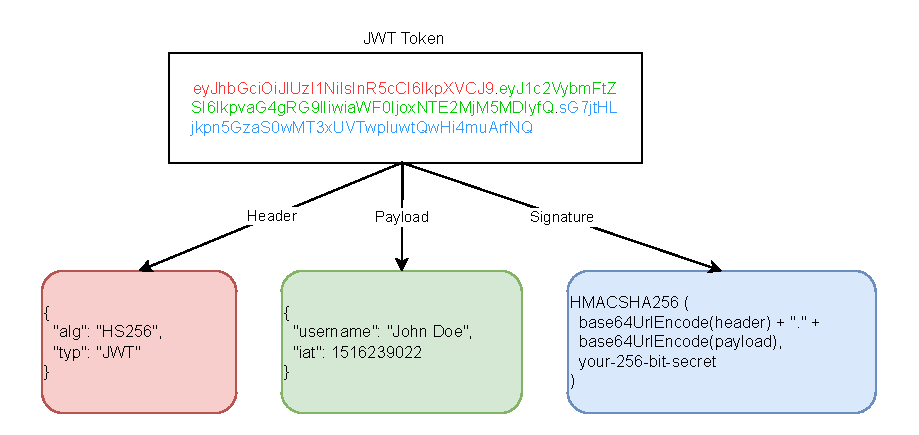
\includegraphics[width=1.1\columnwidth]{graphics/jwt-explained.pdf}
	\end{center}
	
	
		\vspace*{0.5cm}
	\begin{tabular}{ @{} m{0.25\textwidth} m{0.7\textwidth} @{} }
		\begin{minipage}{\linewidth}
			\centering
			
\includegraphics[width=0.5\linewidth]{graphics/redis.png}
			\captionof{figure}{Redis Logo}
			\label{fig:redis}
		\end{minipage}
		&
		\begin{minipage}{\linewidth}
			\textbf{Redis} is an in-memory data structure store, Redis is used for session management, particularly in storing refresh tokens. By caching these tokens, Redis reduces the load on the database and enhances the system’s performance.
		\end{minipage}
	\end{tabular}
	
	
	
	\subsubsection{Database: PostgreSQL}
	
	\begin{figure}[H]
		\centering
		
\includegraphics[scale=0.1]{graphics/postgresql.png}
		\caption{PostgreSQL \acs{rdbms} Logo}
		\label{fig:postgresql}
	\end{figure}
	
	\textbf{PostgreSQL} is a powerful, open-source relational database that offers strong ACID compliance, making it suitable for managing critical data like user accounts, ticket information, and communication logs. Its support for advanced querying and indexing ensures the system can handle complex searches efficiently.
	
	
	\subsubsection{Responsive Web Design: Techniques and Tools}
	
	\begin{itemize}
		\item \textbf{Media Queries}: CSS media queries are used to apply different styles based on device characteristics (screen size, resolution). This allows the frontend to automatically adapt to different devices, ensuring that the system is usable on desktops, laptops, tablets, and smartphones.
		
		\item \textbf{CSS Flexbox/Grid}: These CSS layout models allow for flexible, responsive layouts that adjust to different screen sizes. Flexbox is ideal for managing component positioning in small screens, while Grid is useful for creating complex layouts in larger screens.
	\end{itemize}


\subsection{Theoretical Background}

	\subsubsection{Ticket Management Systems}
	A ticket management system is a tool designed to manage and track the progress of support requests, from the time they are submitted until they are resolved. The system typically assigns a unique identifier (ticket) to each request, enabling staff to monitor progress, prioritize issues, and provide timely responses.
	In a university context, ticket management systems are particularly useful for handling student issues, such as dormitory problems, academic inquiries, and administrative requests. By assigning specific staff members to tickets, the system ensures accountability and reduces response time.
	
	\subsubsection{Real-Time Communication Tools}
	Real-time communication tools like SocketIO or WebSockets are essential in modern web applications. These tools allow for instantaneous data transmission between the server and client, enabling real-time messaging and live updates. For instance, in the Student Life Support Service, students and staff can exchange messages directly without having to refresh the page, ensuring efficient communication.
	
	\subsubsection{Web Application Development Best Practices}
	\begin{itemize}
		\item \textbf{Modular Design}: Applications should be developed in a modular fashion, separating concerns into distinct components (frontend, backend, database). This allows for easier maintenance and scalability.
		
		\item \textbf{Security First}: With the increasing number of security breaches in web applications, implementing security best practices like JWT for authentication, HTTPS for communication, and proper data validation is essential.
		
		\item \textbf{Responsive Design}: Ensuring that the application works across different devices and screen sizes is a fundamental best practice, especially for a university setting where students and staff might use a wide variety of devices.
	\end{itemize}
		
		
\subsection{Gap Analysis}

	\subsubsection{What is Missing from Existing Solutions}
	Existing solutions for university support systems face several shortcomings. Privacy concerns arise in social media-based group chats, where sensitive student information may be exposed, and even proprietary systems lack a strong focus on educational privacy needs. Role-specific functionalities are often missing, with few systems offering specialized tools for students, dormitory staff, or administrators, or including student-centric features like feedback collection, ticket rating, and public status views. Limited analytics is another issue; while general analytics are provided, they don’t cater to the specific needs of student services, such as tracking recurring issues or ticket performance. Additionally, many systems, like JIRA, are not user-friendly for students, requiring training and posing barriers in environments where simplicity is essential.
	
	\subsubsection{How the Student Life Support Service Fills These Gaps}
	The Student Life Support Service addresses the gaps in existing systems by offering a solution tailored specifically to university needs. Its customizable structure supports role-specific functionalities for students, dormitory staff, and administrators, making it ideal for managing university-specific scenarios like dormitory issues and academic inquiries. Real-time communication is enabled through SocketIO, allowing fast, interactive responses between students and staff. The user-friendly interface, built with ReactJS and Material UI, ensures easy navigation for non-technical users. As an open-source, cost-effective platform using NodeJS, PostgreSQL, and ReactJS, it avoids the high costs of proprietary software. The system also provides role-specific features, such as ticket creation, tracking, and rating for students, efficient ticket handling for staff, and detailed reporting tools for administrators. Enhanced privacy and security are ensured through JWT-based authentication and role-based access, preventing unauthorized access to sensitive information. Additionally, built-in data analytics offers administrators insights into ticket trends and areas for improvement in student support services.
	
	
	
			